%!TEX root = ../thesis.tex
This section will focus on describing and discussing a selection of concepts for ad hoc interfaces based on the jamming technique.
As mentioned in the beginning of this chapter we were not successful at implementing a working jamming system where we could effectively control air/liquid flow.
Therefore we concentrate on conceptual prototypes which we envisioned before taking the decision to move in other directions.
Each of these concepts have different focal points.
The first one, \emph{\nameref{ch:jamming:concepts:dynamic_input}}, strives to achieve on-demand standard interfaces for input control.
The second, \emph{\nameref{ch:jamming:concepts:playful_blobs}}, seeks to draw on known interaction metaphors from the digital world and expose them to physical objects.
The third, \emph{\nameref{ch:jamming:concepts:improvised_furniture}}, scales up the dimensions and focuses on a living environment with highly configurable components.

\subsection{Dynamic input controls} 
\label{ch:jamming:concepts:dynamic_input}

This concept was our starting point for our first endeavours with jamming.

The concept resembles the work of \citet{harrison2009providing} mentioned in the related work section and our intentions were also to create physical input controls with the dynamic qualities of the digital counterpart.
But we were of the opinion that by using the jamming technique we could overcome some of the constraints of their approach and offer even more flexibility.
The limitations of the approach taken by \citet{harrison2009providing} were primarily the reliance on a backing layer where cut-out areas determined the position and shape of the buttons.
They were able to show a button either in convex or concave form or not at all, but the buttons were locked in their positions and the shapes were also not modifiable.

Instead, we propose using the jamming technique with a cell-based approach.
Individual cells can be used to create deformations on different areas of the surface and the composition of multiple cells makes it possible to make forms of heterogeneous shapes emerge anywhere on the plane, see figure \ref{fig:ch:jamming:concepts:button-cells}.
The idea of composition is quite similar to the that of computer graphics where polygons are used to compose images that are appear three-dimensional.
In this way, not only can we make input controls appear and disappear, we can also change the shape and position of them for an even more dynamic interface.

As a simple example we made mocked up a prototype to demonstrate simple shapes by jamming.
Due to our issues with a jamming, this was again a setup with a vacuum cleaner, plastic bag as the membrane, and ground coffee as the particles, see figure \ref{fig:ch:jamming:concepts:inputs-prototype}.

\begin{figure}[h]
  \centering
  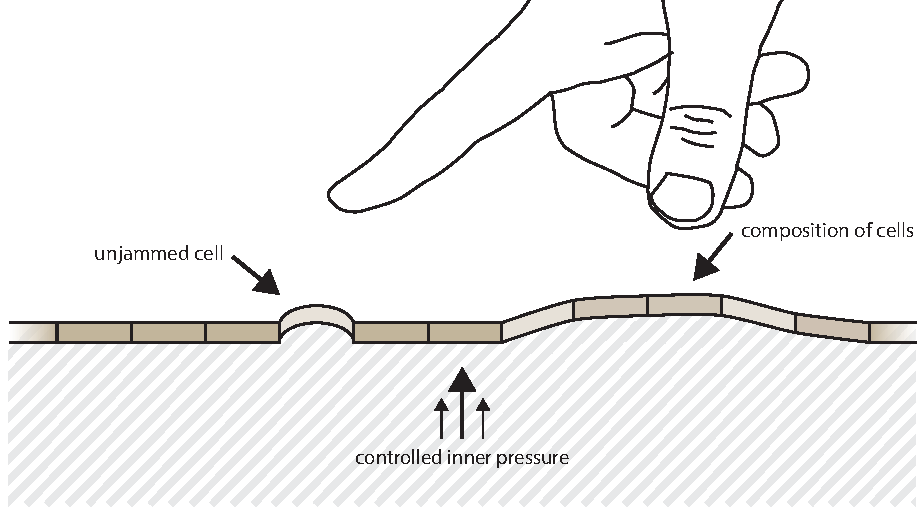
\includegraphics[width=.9\textwidth]{figures/jamming/concepts/jamming-inputs-concept.pdf}
  \caption{A cross-sectional view of a cell-based button and a composition multiple cells with different pressures for complex forms.}
  \label{fig:ch:jamming:concepts:button-cells}
\end{figure}

%We conceptualize on household appliances such as radios, clock alarms, house alarms heating, ventilation and air conditioning (HVAC), \todo{etc}.
%In general physical products with standard input controls such as buttons, knobs, switches and sliders.

\begin{figure}[h]
\centering
\begin{subfigure}[t]{.44\textwidth}
  \centering
  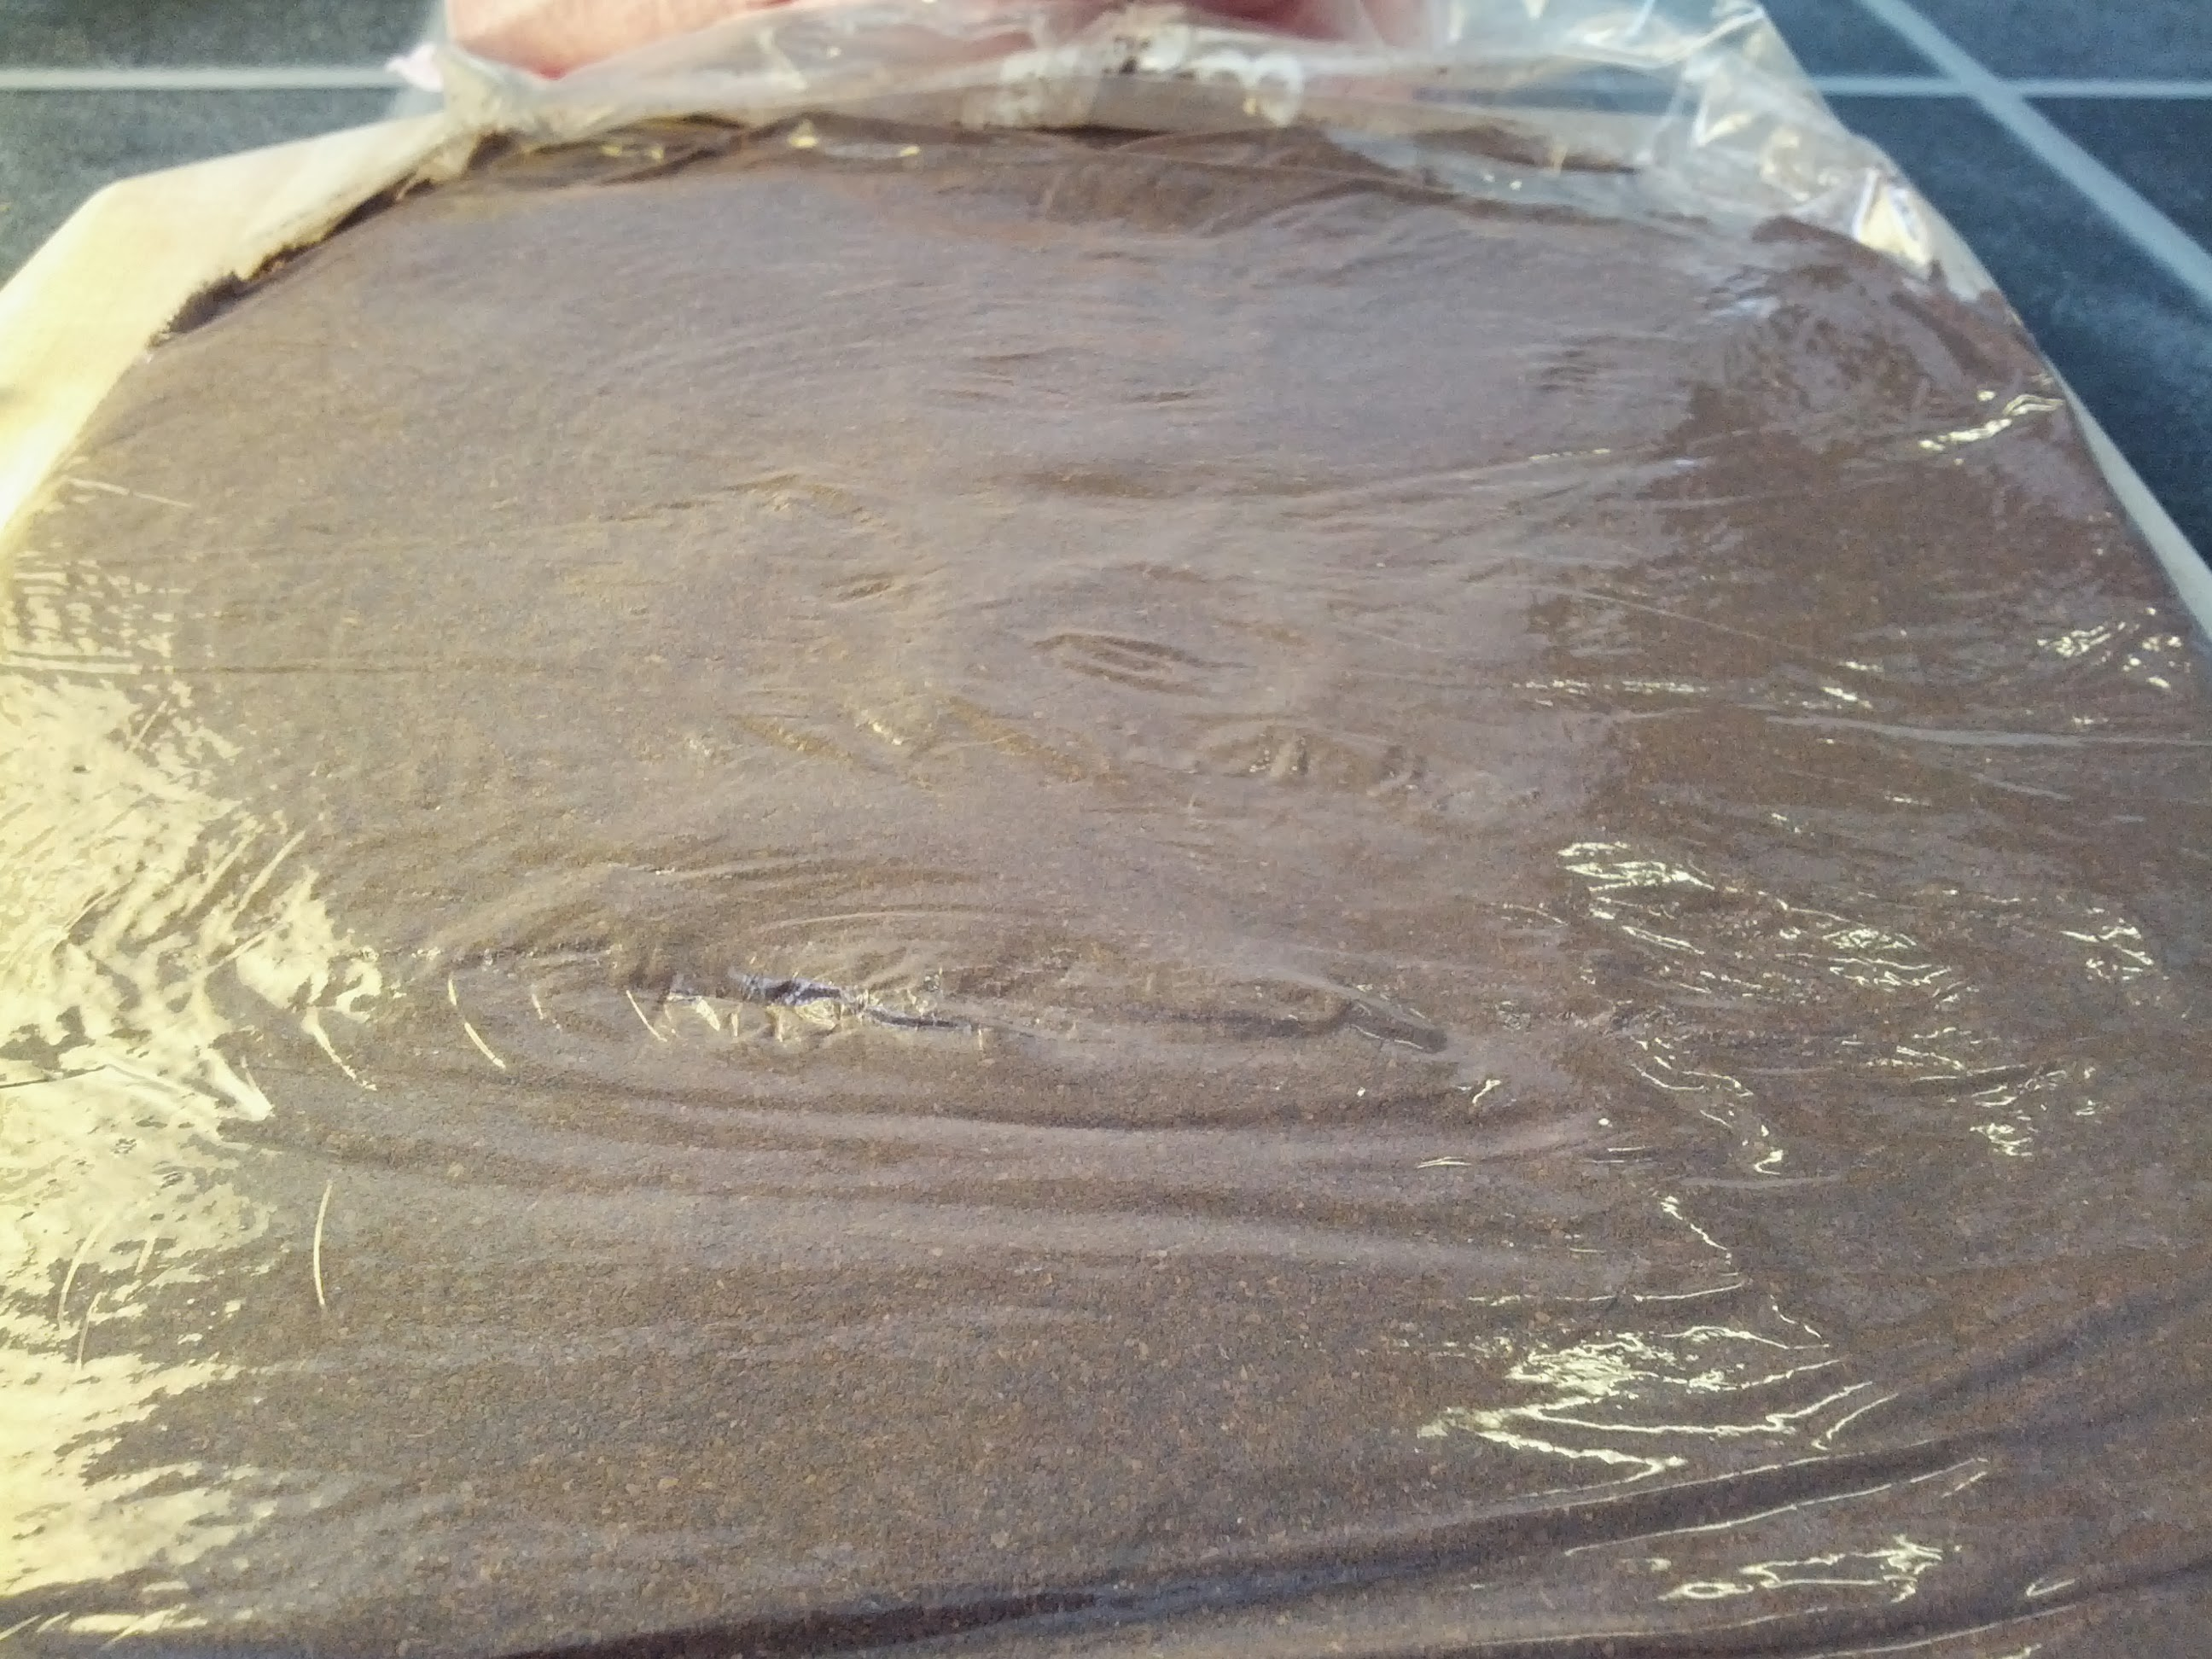
\includegraphics[width=\linewidth]{figures/jamming/concepts/inputs/jamming-inputs-flat}
    \caption{A flat surface with the absence of any input controls.}
\end{subfigure}%
\hspace{0.02\textwidth}
\begin{subfigure}[t]{.44\textwidth}
  \centering
  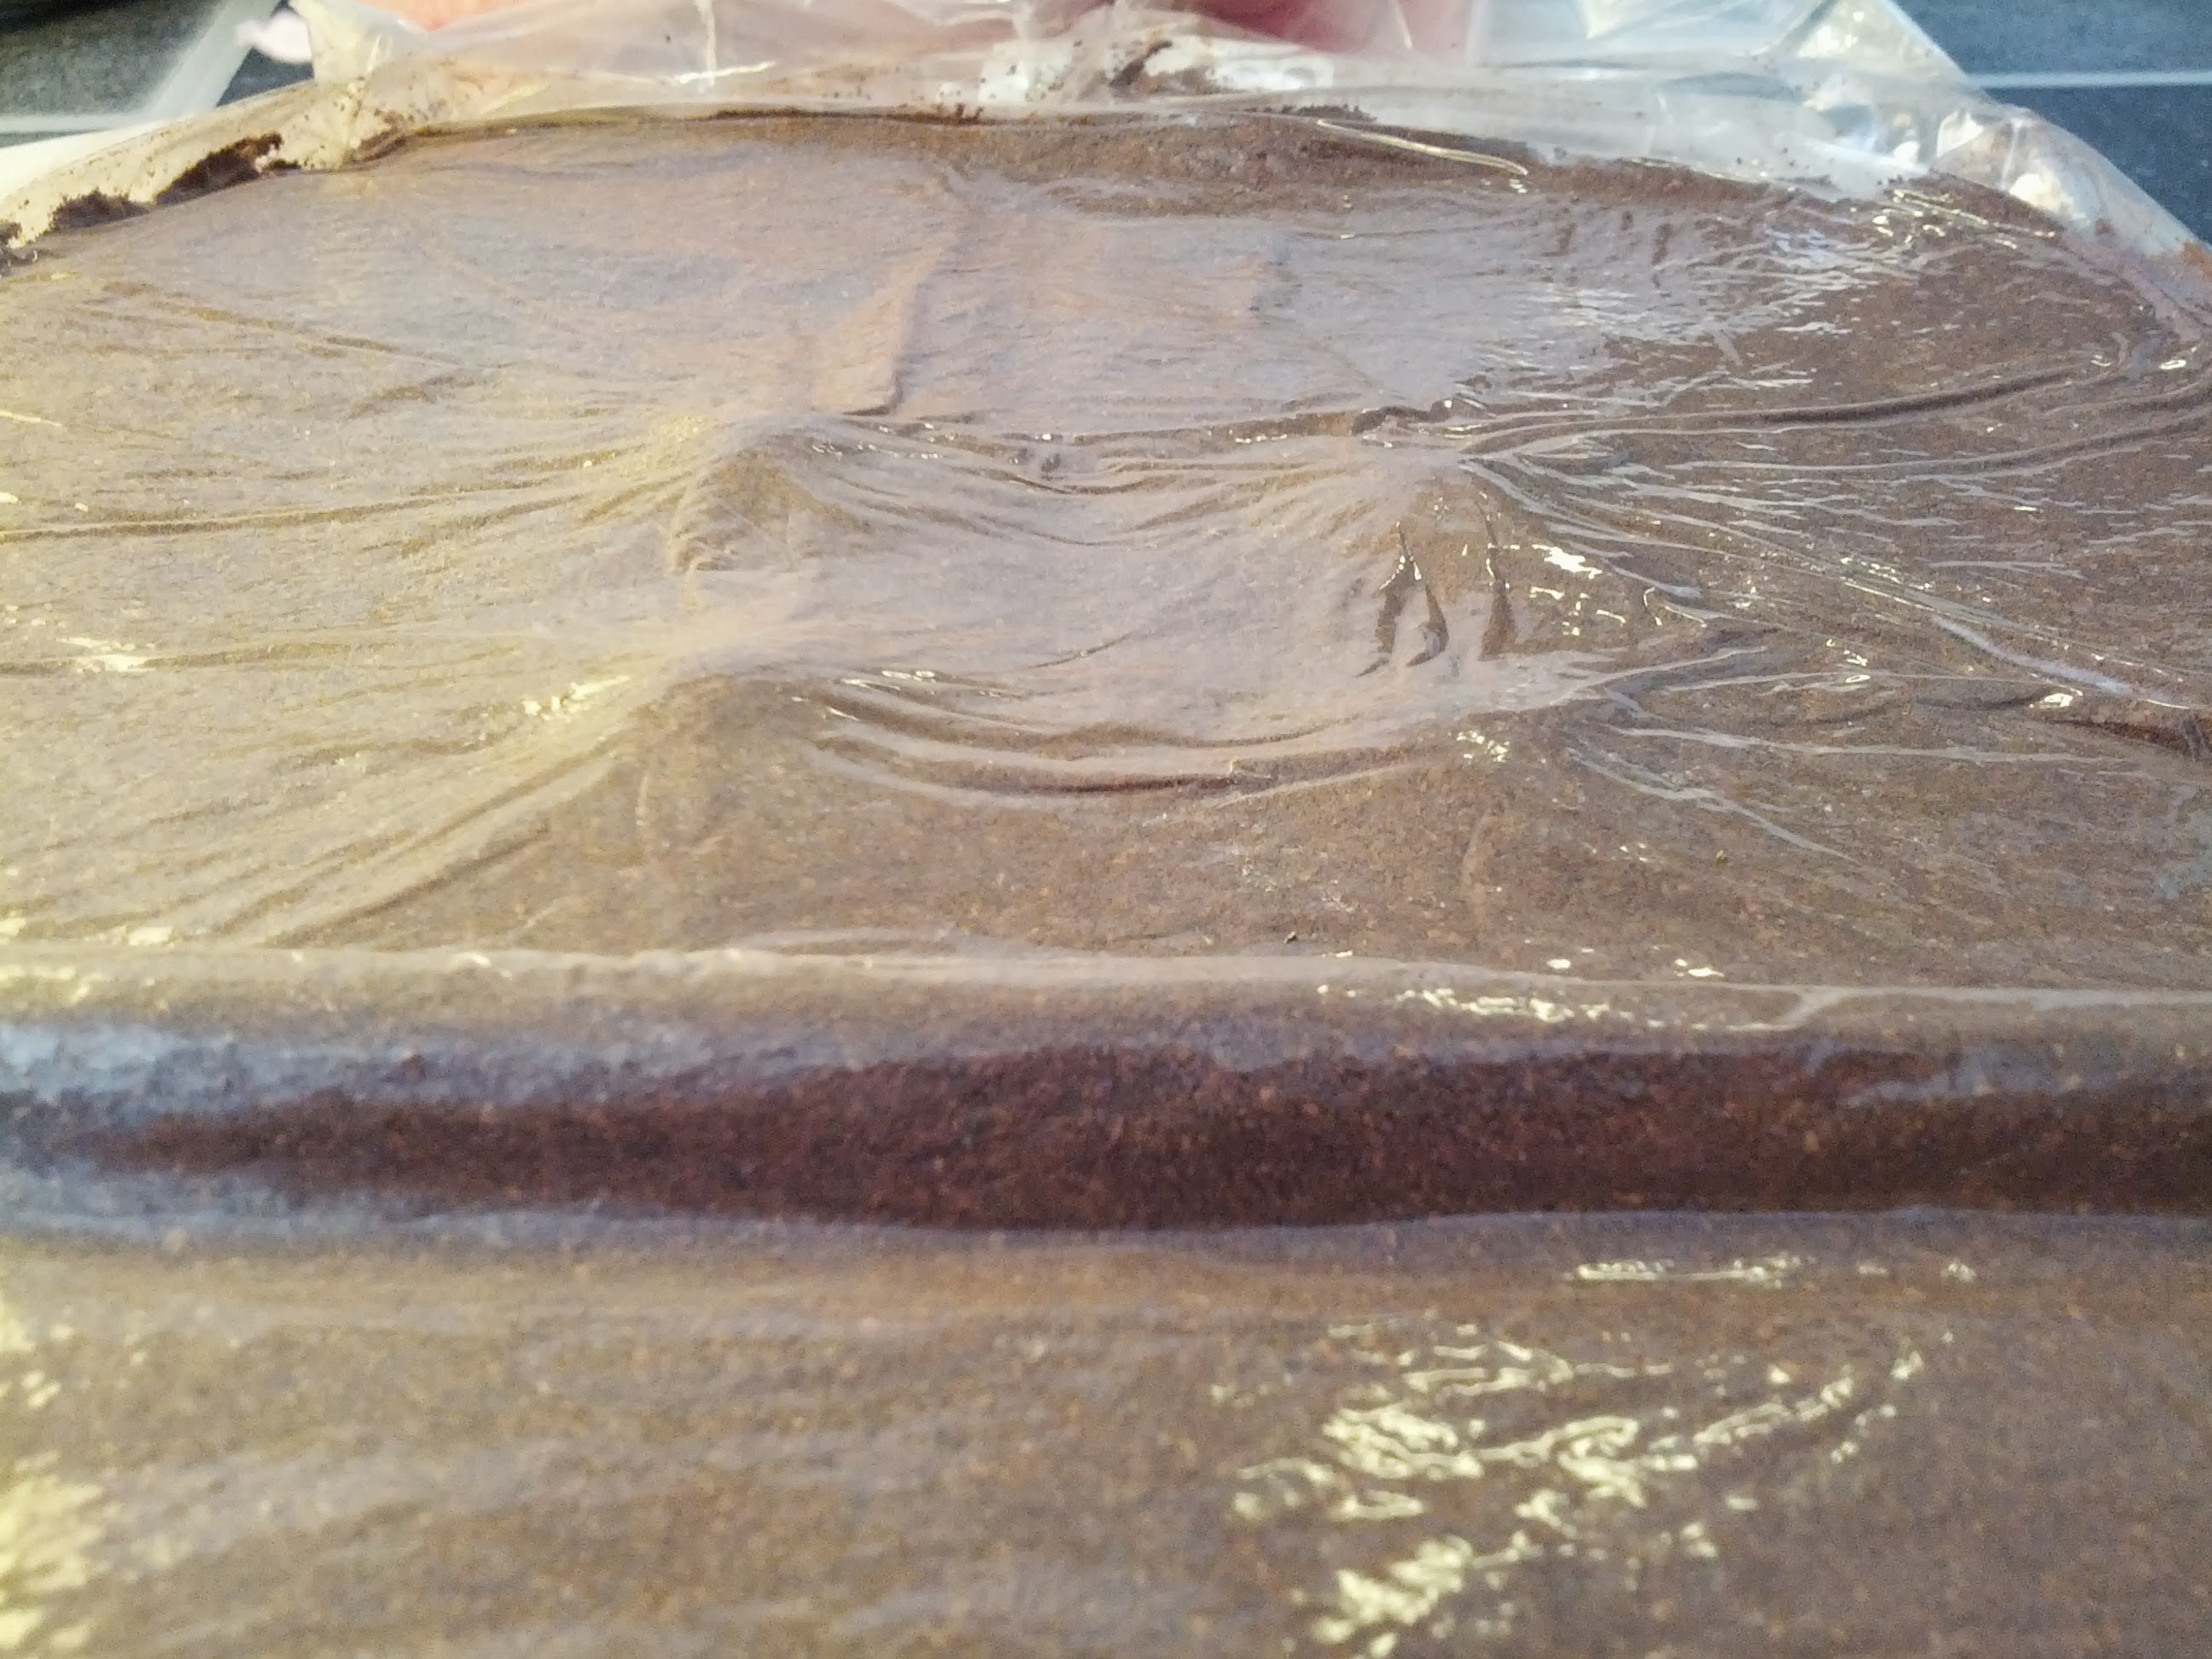
\includegraphics[width=\linewidth]{figures/jamming/concepts/inputs/jamming-inputs-buttons}
  \caption{Four buttons have emerged and an elongated input control for e.g. sliding or grabbing and pulling.}
\end{subfigure}
\caption{A primitive exploratory prototype with basic jamming of a single volume. Ground coffee is enclosed withing a transparent plastic bag. Wrinkles occur due to the plastic bag not being very flexible.}
\label{fig:ch:jamming:concepts:inputs-prototype}
\end{figure}

\subsection{Playful blobs}
\label{ch:jamming:concepts:playful_blobs}

The focal point of this next concept is on bringing input and output into the same object.
As can be seen in table~\ref{ch:jamming:table:applications_overview} on page~\pageref{ch:jamming:table:applications_overview} only one of the listed projects from the related work section, \nameref{fig:ch:jamming:jui-tablet}, has both input and output in same object.
Therefore we see an unexplored area of jamming potentials which we would like to address in the this next concept.

We envision a toy concept for children which we call \nameref{ch:jamming:concepts:playful_blobs}.
The blobs are tangible clay-like objects meant to be moulded into creative forms.
Each blob makes a selection of commands available otherwise known from digital interface metaphors, such as \emph{save, open, undo, delete, copy, and paste} which can actuate the blob in different ways.
These commands give a physical blob a notion of form memory where state is kept over time.
If needed previously saved forms can be recalled and further work on the form can done.
More specifically each command means (see also figure~\ref{fig:ch:jamming:concepts:blobs:states}):
\begin{itemize}
	\item{\emph{Save}: The current form of a blob is saved in memory for later retrieval.}
	\item{\emph{Open}: A previously saved form can be recalled and the blob actuates itself into the saved state.}
	\item{\emph{Undo}: Negate the latest moulding of the blob.}
	\item{\emph{Copy}: Make a copy of the state of a specific blob. The copied state could be saved in a blob or in an external object.}
	\item{\emph{Paste}: Set the state of a blob to that of which has been copied.} 
	\item{\emph{Delete}: Reset a blob so that all state is forgotten.} 
\end{itemize}

\begin{figure}[h]
  \centering
  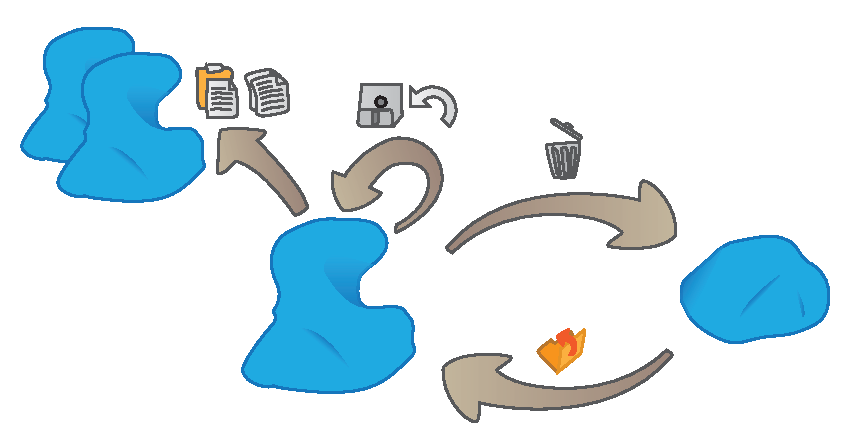
\includegraphics[width=.9\textwidth]{figures/jamming/concepts/blobs/state-transitions.pdf}
  \caption{A visualisation of the different commands}
  \label{fig:ch:jamming:concepts:blobs:states}
\end{figure}

The commands are made possible via a cell-based jamming structure and the amount of detail a moulded blob can have is dictated by the resolution of the jamming cells.
As mentioned earlier this jamming approach makes it possible to separately control the stiffness of each cell.
So, for example, the \emph{save} command is done by storing a map of the current pressure states of each cell.
A subsequent \emph{open} or \emph{paste} command would set the correct pressure values of the cells and thereby restore the \emph{saved} or \emph{copied} physical form.
Lastly, a \emph{delete} command would release all negative pressure in cells and thereby collapse the form.
A simple prototype is shown figure~\ref{fig:ch:jamming:concepts:blobs:gloves} made with the basic jamming approach.
The actuation process would have to be done in a correct sequence in order for specific curvatures to become possible, which presumably could be done by computation.

\begin{figure}[h]
  \centering
  \begin{subfigure}[t]{.28\textwidth}
    \centering
    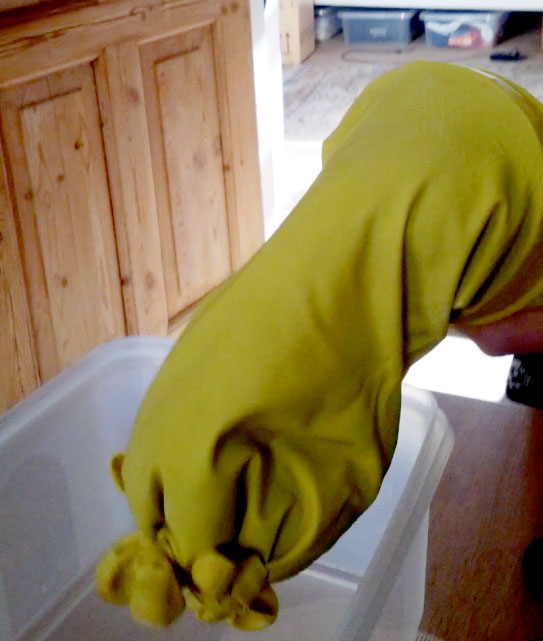
\includegraphics[width=\linewidth]{figures/jamming/concepts/blobs/glove-1.jpg}
    \captionof{figure}{The blob in collapsed state, i.e. no pressure is upheld.}
    \label{fig:ch:jamming:concepts:blobs:g1}
  \end{subfigure}%
  \hspace{0.03\textwidth}
  \begin{subfigure}[t]{.28\textwidth}
    \centering
    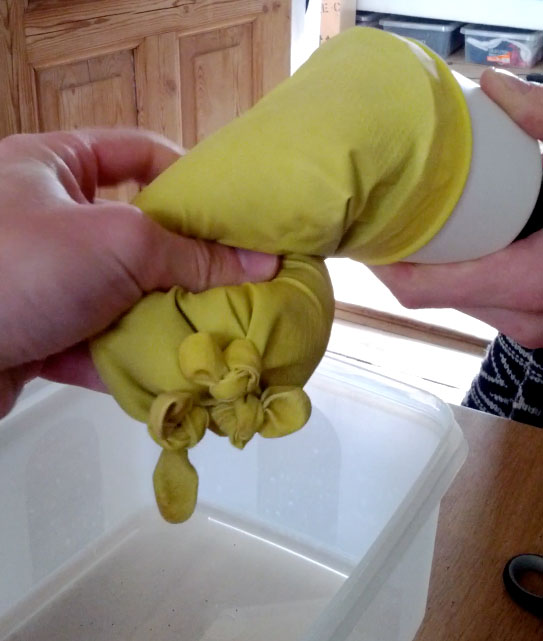
\includegraphics[width=\linewidth]{figures/jamming/concepts/blobs/glove-2}
    \captionof{figure}{The blob being molded into a custom shape.}
    \label{fig:ch:jamming:concepts:blobs:g2}
  \end{subfigure}
  \hspace{0.03\textwidth}
  \begin{subfigure}[t]{.28\textwidth}
    \centering
    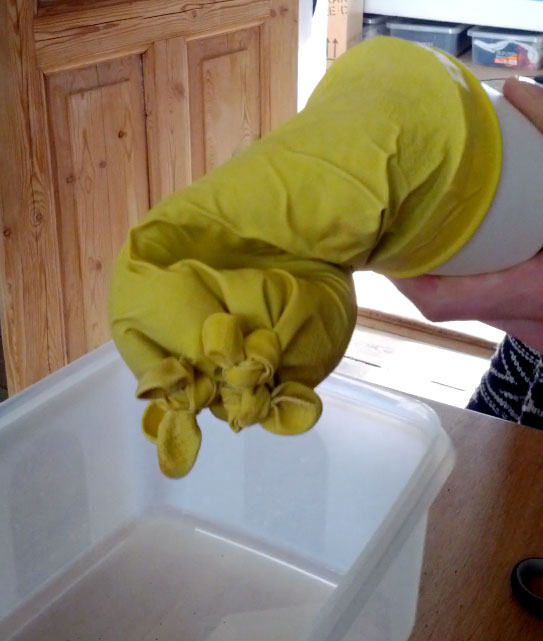
\includegraphics[width=\linewidth]{figures/jamming/concepts/blobs/glove-3}
    \captionof{figure}{The shape of the blob is maintained.} 
    \label{fig:ch:jamming:concepts:blobs:g3}
  \end{subfigure}
  \caption{An exploratory prototype of playful blobs. Created with a rubber latex glove, ground coffee, and a vacuum cleaner. For a video of the above steps see appendix~\ref{app:videos:jamming} which also shows the rigidity of the shape when jammed.}
  \label{fig:ch:jamming:concepts:blobs:gloves}
\end{figure}

We envision that the blobs can be used in a clay-like manner for kids to explore moulding of material into various forms and where particular interesting forms can be saved, duplicated and so on.
Furthermore, we also envision that these blobs could be used as the foundation for a new kind of dynamic building block for construction toys.
A concept that takes products such as Lego\footnote{http://www.lego.com/} a step further by having building blocks that are deformable and can be locked into any shape by the use of jamming.
This allows for block shapes that are no more limited to the supply of the production company but which allow for custom moulded blocks that are adapted to the needs of the user.

Applying these digital features to the physical blobs exhibits ad hoc qualities where the shape itself forms the interface and where shapes can be created on an ad hoc basis.
When a particular shape is no longer needed it can disappear again by remoulding it or letting it collapse (jamming-wise).

\subsection{Improvised furniture}
\label{ch:jamming:concepts:improvised_furniture}

This concept is based on replacing static components of the home with dynamic jamming enabled substitutes.
In its most extreme case with a large scale deployment it may be a little far fetched but an intriguing thought experiment and maybe not that unrealistic in a more futuristic scenario.
It underpins the idea of a configurable home where otherwise static and massive components such as walls and furniture allow for deformations.
For example, pushing in part of a wall to make room for a plant or even an entire shelf.
Or, deforming the floor to improvise an extra seat for a guest.
Or, adjusting the armrest or back of the sofa for a more comfortable position.

These examples correlate with what we touched upon in \autoref{ch:domain} about Steward Brands understanding of changes in a building;
Pulling down a given layer of change to a lower layer to create a more dynamic and adaptable environment.
The concept of improvised furniture would then be \emph{Space Plan} elements that are exposed to the layer of \emph{Stuff}. 
Figure~\ref{fig:ch:jamming:concepts:impro} illustrates deformation of walls for improvised furniture.

With this reconfigurability done by hand the components will naturally end up having an organic appearance with curvatures and very few straight lines and edges.

Using jamming in a large scale deployment where strength and bearing capacity is a requirement does come with quite a few constraints regarding materials.
The container of the particles must be strong enough to handle the exposed level of stress and strain while still being flexible enough to allow for surface deformations.

\begin{figure}[h]
  \centering
  \begin{subfigure}[t]{.44\textwidth}
    \centering
    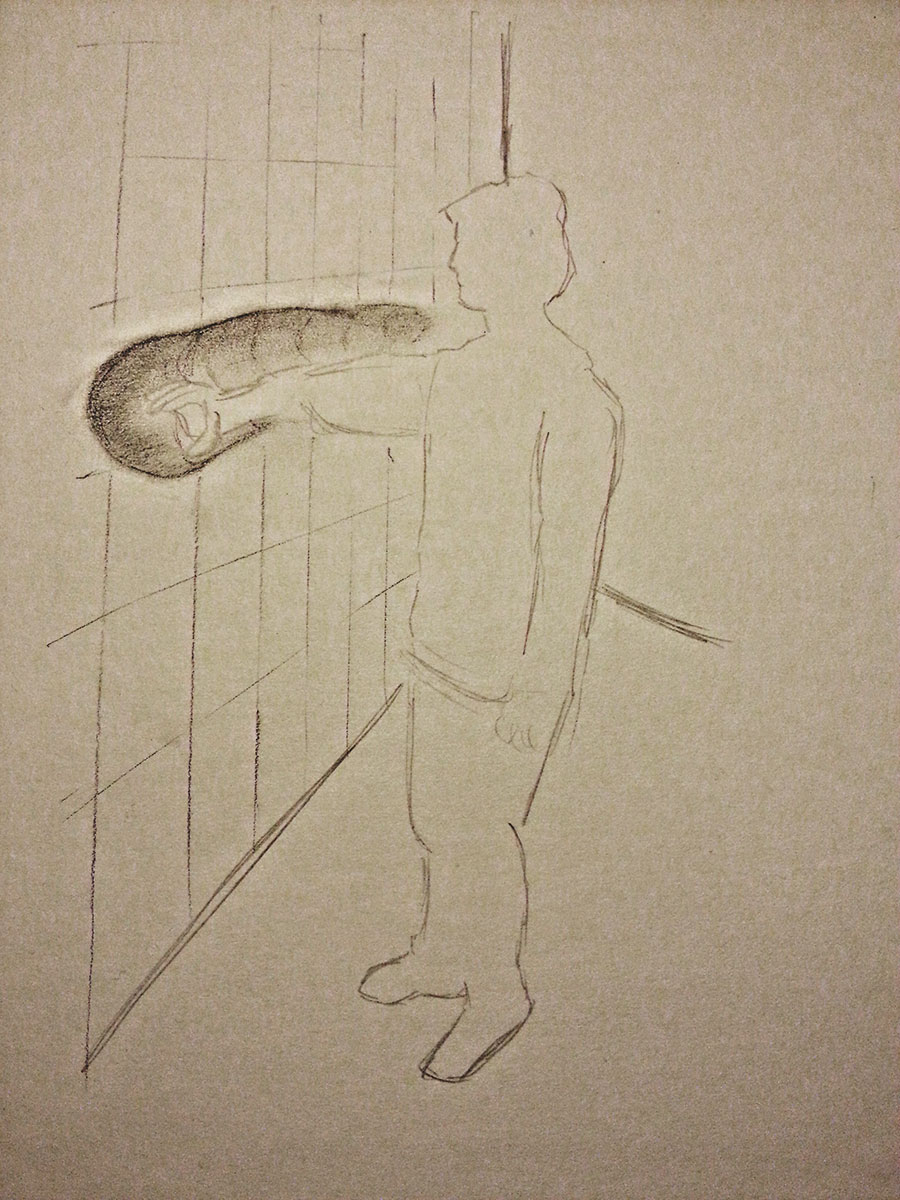
\includegraphics[width=\linewidth]{figures/jamming/concepts/impro/carve}
    \caption{...}
  \end{subfigure}%
  \hspace{0.02\textwidth}
  \begin{subfigure}[t]{.44\textwidth}
    \centering
    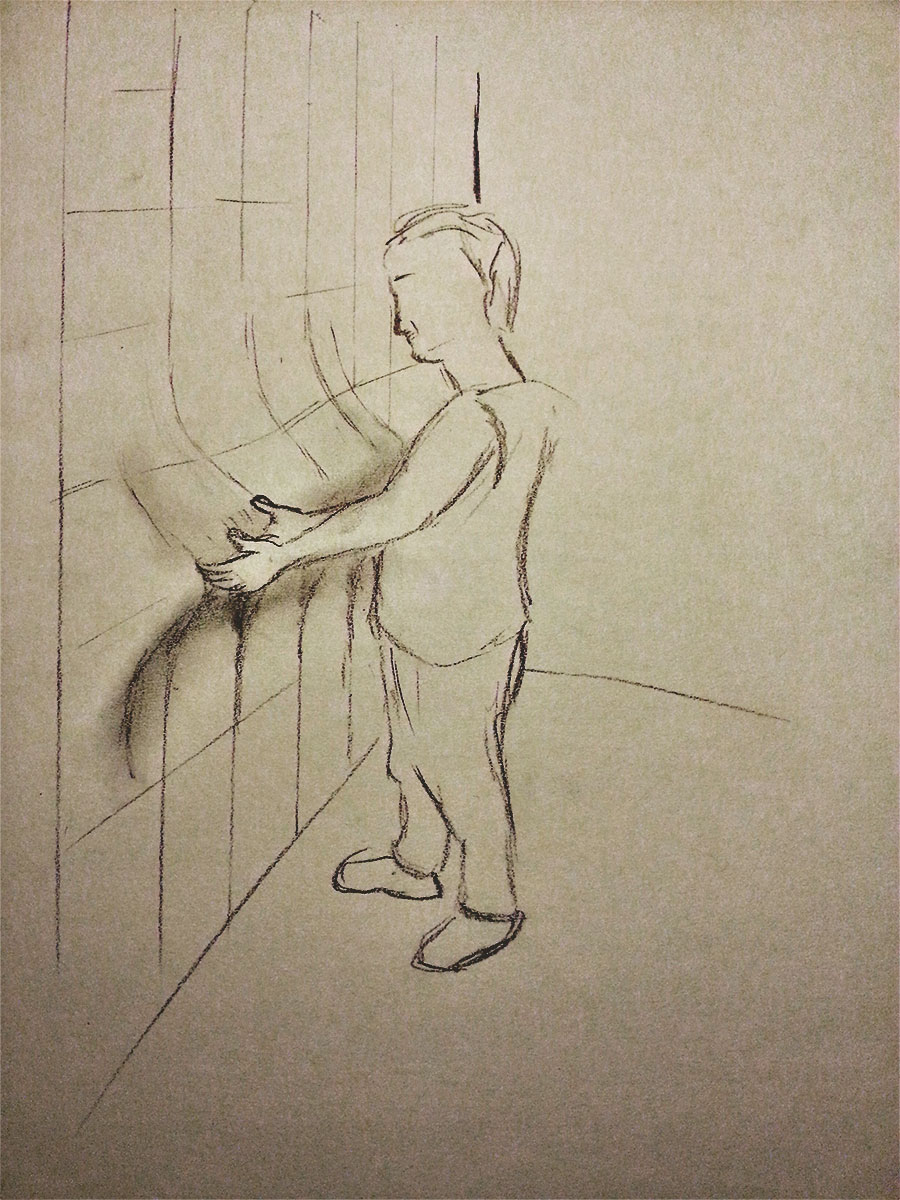
\includegraphics[width=\linewidth]{figures/jamming/concepts/impro/pull}
    \caption{...}
  \end{subfigure}
  \caption{...}
\label{fig:ch:jamming:concepts:impro}
\end{figure}

